\documentclass{article}
\newtheorem{thm}{Theorem}
\setlength{\oddsidemargin}{0.25in}
\setlength{\textwidth}{6in}
\setlength{\topmargin}{-0.25in}
\setlength{\headheight}{0.3in}
\setlength{\headsep}{0.2in}
\setlength{\textheight}{9in}
\setlength{\footskip}{0.1in}
\usepackage{multirow}
\usepackage{fullpage}
\usepackage{graphicx}
\usepackage{amsthm}
\usepackage{amssymb}
\usepackage{url}
\usepackage{amsfonts}
\usepackage{algpseudocode}
\usepackage{mathtools}
\usepackage{float}
\usepackage{listings}
\usepackage{color}
 
\definecolor{codegreen}{rgb}{0,0.6,0}
\definecolor{codegray}{rgb}{0.5,0.5,0.5}
\definecolor{codepurple}{rgb}{0.58,0,0.82}
\definecolor{backcolour}{rgb}{0.95,0.95,0.92}
 
\lstdefinestyle{mystyle}{
    backgroundcolor=\color{backcolour},   
    commentstyle=\color{codegreen},
    keywordstyle=\color{magenta},
    numberstyle=\tiny\color{codegray},
    stringstyle=\color{codepurple},
    basicstyle=\footnotesize,
    breakatwhitespace=false,         
    breaklines=true,                 
    captionpos=b,                    
    keepspaces=true,                 
    numbers=left,                    
    numbersep=5pt,                  
    showspaces=false,                
    showstringspaces=false,
    showtabs=false,                  
    tabsize=2
}
 
\lstset{style=mystyle}

\begin{document}\title{Project 8: Harp Mini\-Batch Kmeans\\ Cloud Computing\\ Spring 2017}         % Enter your title between curly braces
\author{Professor Judy Qiu }        % Enter your name between curly braces
\date{}
%\date{\today}          % Enter your date or \today between curly braces
\maketitle
\makeatother     % `@' is restored as a "non-letter" character
\pagestyle{plain}
\section*{Goal}
The goal for this project is to implement Harp\cite{Harp} Mini-batch Kmeans from scratch. 

\section*{Deliverables}
Zip your source code and report as username\_mbkmeans.zip. Please submit this file to the Canvas Assignments page.

\section*{Evaluation}

The point total for this project is 6, where the distribution is as follows:
\begin{itemize}
\item Completeness of your code (5 points)
\item In the report, describe your implementation and the output. (1 points)
\end{itemize}
 You can get up to 4 bonus points based on your  extra efforts.
\section*{Bonus credits}

Some options you may consider to get extra credits: 
\begin{itemize}
\item Perform experiments on various (small, medium, large, etc) datasets 
\item Test your algorithm on at least 2 nodes on FutureSystem.
\item Implement mini-batch kmeans using other tools/platforms (Spark\cite{Spark}, Flink\cite{Flink}, etc) and compare the performance between different tools/platforms.
\end{itemize}
You are encouraged to explore other options to get extra credits. Remember to present all of your extra work in the report.
 
\section*{Dataset}
You can implement a script to  generate data randomly as your input datasets.  You are also free to use public datasets such as RCV1-v2\cite{RCV1-v2}.
  
\section*{Mini-batch Kmeans}
You can refer to the paper\cite{sculley2010web} for sequential mini-batch kmeans algorithm. You will need to design how to parallelize the algorithm so that it can run with large scale datasets on distributed computing environment.

\begin{figure}[H]
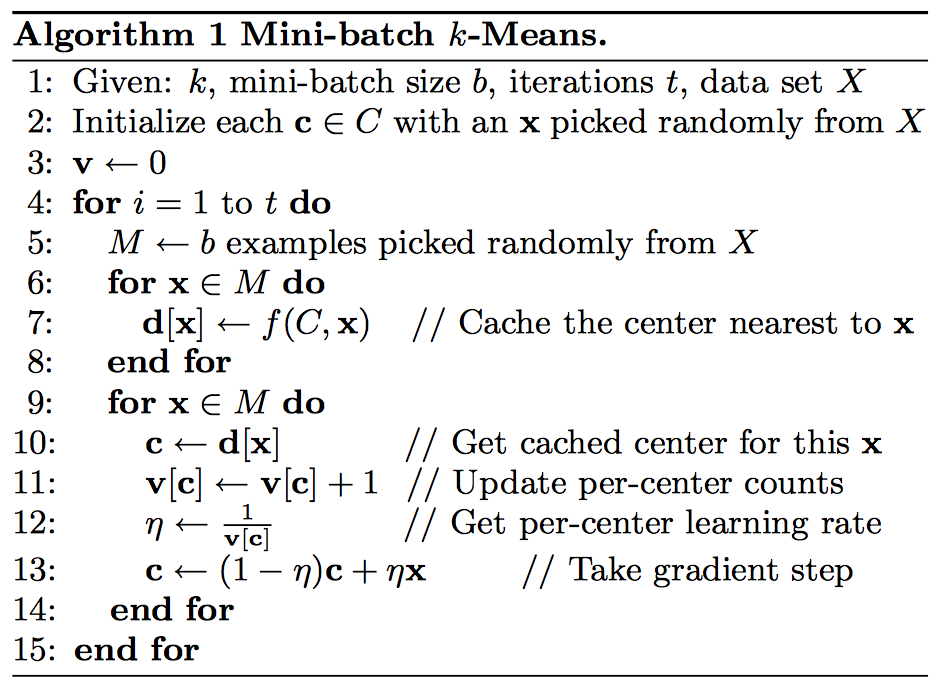
\includegraphics[width=8cm]{mbkmeans}
\centering
\caption{Mini-batch Kmeans.\cite{sculley2010web} }
\end{figure}  




\bibliography{mbkmeans} 
\bibliographystyle{unsrt} 
\end{document}
